\begin{figure}[t]
  \centering
  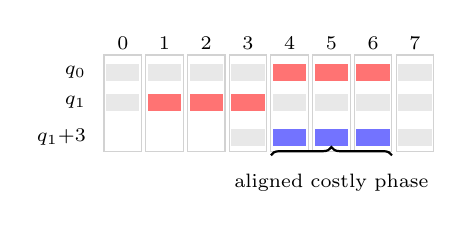
\begin{tikzpicture}[font=\scriptsize, x=5.3mm, y=5mm]
    \foreach \x in {0,...,7} {
      \node at (\x,1.75) {\x};
      \draw[gray!35] (\x-0.45,-1.0) rectangle (\x+0.45,1.45);
    }
    \node[anchor=east] at (-0.65,1) {$q_0$};
    \node[anchor=east] at (-0.65,0.25) {$q_1$};
    \foreach \x in {0,...,7} \fill[gray!18] (\x-0.4,0.78) rectangle (\x+0.4,1.22);
    \foreach \x in {0,...,7} \fill[gray!18] (\x-0.4,0.03) rectangle (\x+0.4,0.47);
    \foreach \x in {4,5,6} \fill[red!55] (\x-0.4,0.78) rectangle (\x+0.4,1.22);
    \foreach \x in {1,2,3} \fill[red!55] (\x-0.4,0.03) rectangle (\x+0.4,0.47);
    \node[anchor=east] at (-0.65,-0.65) {$q_1{+}3$};
    \foreach \x in {3,...,7} \fill[gray!18] (\x-0.4,-0.87) rectangle (\x+0.4,-0.43);
    \foreach \x in {4,5,6} \fill[blue!55] (\x-0.4,-0.87) rectangle (\x+0.4,-0.43);
    \draw[decorate, decoration={brace, amplitude=3pt}, thick]
      (3.55,-1.1) -- (6.45,-1.1) node[midway, below=3pt] {aligned costly phase};
  \end{tikzpicture}
  \caption{Why start offsets can increase sharing.  Red cells denote expensive traversal phases that do not overlap at zero offset; delaying $q_1$ by three global iterations aligns them (blue).  The offset changes time, not either query's logical levels.}
  \Description{Two query timelines have expensive phases at different global steps.  Delaying the second query shifts its expensive phase to coincide with the first.}
  \label{fig:phase-alignment}
\end{figure}
